
%<<setup-child, include = FALSE>>=
%library(knitr)
%set_parent("../style/preamble.Rnw")
%@
\input{../../2021/style/preamble4tex}
% dependencies: amsmath, amssymb, dsfont
% math spaces
\ifdefined\N
\renewcommand{\N}{\mathds{N}} % N, naturals
\else \newcommand{\N}{\mathds{N}} \fi
\newcommand{\Z}{\mathds{Z}} % Z, integers
\newcommand{\Q}{\mathds{Q}} % Q, rationals
\newcommand{\R}{\mathds{R}} % R, reals
\ifdefined\C
\renewcommand{\C}{\mathds{C}} % C, complex
\else \newcommand{\C}{\mathds{C}} \fi
\newcommand{\continuous}{\mathcal{C}} % C, space of continuous functions
\newcommand{\M}{\mathcal{M}} % machine numbers
\newcommand{\epsm}{\epsilon_m} % maximum error

% counting / finite sets
\newcommand{\setzo}{\{0, 1\}} % set 0, 1
\newcommand{\setmp}{\{-1, +1\}} % set -1, 1
\newcommand{\unitint}{[0, 1]} % unit interval

% basic math stuff
\newcommand{\xt}{\tilde x} % x tilde
\newcommand{\argmin}{\mathop{\mathrm{arg\,min}}} % argmin
\newcommand{\argmax}{\mathop{\mathrm{arg\,max}}} % argmax
\newcommand{\argminlim}{\argmin\limits} % argmin with limits
\newcommand{\argmaxlim}{\argmax\limits} % argmax with limits
\newcommand{\sign}{\operatorname{sign}} % sign, signum
\newcommand{\I}{\mathbb{I}} % I, indicator
\newcommand{\order}{\mathcal{O}} % O, order
\newcommand{\bigO}{\mathcal{O}} % Big-O Landau
\newcommand{\littleo}{{o}} % Little-o Landau
\newcommand{\pd}[2]{\frac{\partial{#1}}{\partial #2}} % partial derivative
\newcommand{\floorlr}[1]{\left\lfloor #1 \right\rfloor} % floor
\newcommand{\ceillr}[1]{\left\lceil #1 \right\rceil} % ceiling
\newcommand{\indep}{\perp \!\!\! \perp} % independence symbol

% sums and products
\newcommand{\sumin}{\sum\limits_{i=1}^n} % summation from i=1 to n
\newcommand{\sumim}{\sum\limits_{i=1}^m} % summation from i=1 to m
\newcommand{\sumjn}{\sum\limits_{j=1}^n} % summation from j=1 to p
\newcommand{\sumjp}{\sum\limits_{j=1}^p} % summation from j=1 to p
\newcommand{\sumik}{\sum\limits_{i=1}^k} % summation from i=1 to k
\newcommand{\sumkg}{\sum\limits_{k=1}^g} % summation from k=1 to g
\newcommand{\sumjg}{\sum\limits_{j=1}^g} % summation from j=1 to g
\newcommand{\summM}{\sum\limits_{m=1}^M} % summation from m=1 to M
\newcommand{\meanin}{\frac{1}{n} \sum\limits_{i=1}^n} % mean from i=1 to n
\newcommand{\meanim}{\frac{1}{m} \sum\limits_{i=1}^m} % mean from i=1 to n
\newcommand{\meankg}{\frac{1}{g} \sum\limits_{k=1}^g} % mean from k=1 to g
\newcommand{\meanmM}{\frac{1}{M} \sum\limits_{m=1}^M} % mean from m=1 to M
\newcommand{\prodin}{\prod\limits_{i=1}^n} % product from i=1 to n
\newcommand{\prodkg}{\prod\limits_{k=1}^g} % product from k=1 to g
\newcommand{\prodjp}{\prod\limits_{j=1}^p} % product from j=1 to p

% linear algebra
\newcommand{\one}{\bm{1}} % 1, unitvector
\newcommand{\zero}{\mathbf{0}} % 0-vector
\newcommand{\id}{\bm{I}} % I, identity
\newcommand{\diag}{\operatorname{diag}} % diag, diagonal
\newcommand{\trace}{\operatorname{tr}} % tr, trace
\newcommand{\spn}{\operatorname{span}} % span
\newcommand{\scp}[2]{\left\langle #1, #2 \right\rangle} % <.,.>, scalarproduct
\newcommand{\mat}[1]{\begin{pmatrix} #1 \end{pmatrix}} % short pmatrix command
\newcommand{\Amat}{\mathbf{A}} % matrix A
\newcommand{\Deltab}{\mathbf{\Delta}} % error term for vectors

% basic probability + stats
\renewcommand{\P}{\mathds{P}} % P, probability
\newcommand{\E}{\mathds{E}} % E, expectation
\newcommand{\var}{\mathsf{Var}} % Var, variance
\newcommand{\cov}{\mathsf{Cov}} % Cov, covariance
\newcommand{\corr}{\mathsf{Corr}} % Corr, correlation
\newcommand{\normal}{\mathcal{N}} % N of the normal distribution
\newcommand{\iid}{\overset{i.i.d}{\sim}} % dist with i.i.d superscript
\newcommand{\distas}[1]{\overset{#1}{\sim}} % ... is distributed as ...



\begin{document}

\lecturechapter{2}{Character Encoding}
\lecture{Computerintensive Methods}

%\section{Character encoding}

% \begin{vbframe}{Example: $e^x$}
% series representation:
% $$
%   e^x = \sum_{n=0}^\infty \frac{x^n}{n !}
% $$

% Does the following code work \pkg{R}?

%<<echo = TRUE, eval = FALSE, include = FALSE>>==
%oldsum = 0
%newsum = n = term = 1
%while(oldsum != newsum){
%  oldsum = newsum
%  term = term * x / n
%  n = n + 1
%  newsum = oldsum + term
%}
%@
% \end{vbframe}


% \begin{vbframe}{Beispiel: $e^x$}
%<<include=FALSE>>=
%opts_chunk$set(size = "scriptsize")
%@

%<<echo = TRUE, include = FALSE>>=
%x = 1
%oldsum = 0
%newsum = n = term = 1
%while(oldsum != newsum){
%  oldsum = newsum
%  term = term * x / n
%  n = n + 1
%  newsum = oldsum + term
%}
%newsum; exp(1)
%term; term + 1.3
%@

% \end{vbframe}

\begin{vbframe}{Bits and Bytes}
\begin{itemize}
\item On digital computers, all information is represented in strings of $0$'s and $1$'s.
\item A single $0$/$1$ digit is called \textbf{bit} (\enquote{binary} + \enquote{digit}).
\item To represent text, bits are usually arranged in groups of eight, in so-called \textbf{bytes}.
\end{itemize}

\begin{center}
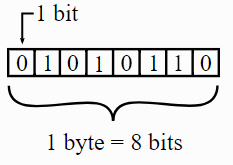
\includegraphics[width=0.4\textwidth]{figure_man/bitbyte.png}
\end{center}


\end{vbframe}

\begin{vbframe}{Codes for character sets: example ASCII}

%\vspace*{-.5cm}
\begin{itemize}
\item The most common code  ASCII (American Standard Code for Information Interchange):
  \begin{itemize}
    \item 95 printable characters.
    \item Bit pattern consists of only $7$ bits.
  \end{itemize}
\end{itemize}

\lz

Wikipedia:

\emph{ASCII, abbreviated from American Standard Code for Information Interchange, is a character-encoding scheme.
ASCII codes represent text in computers, communications equipment, and other devices that use text.
Most modern character-encoding schemes are based on ASCII, though they support many additional characters.
ASCII was the most common character encoding on the World Wide Web until December 2007, when it was surpassed by UTF-8, which includes ASCII as a subset.}

\framebreak

\begin{center}
\begin{tabular}{l}
% $\,\,$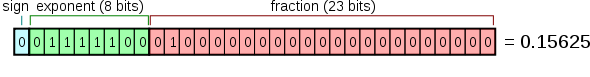
\includegraphics{32bit} \\[0.15cm]
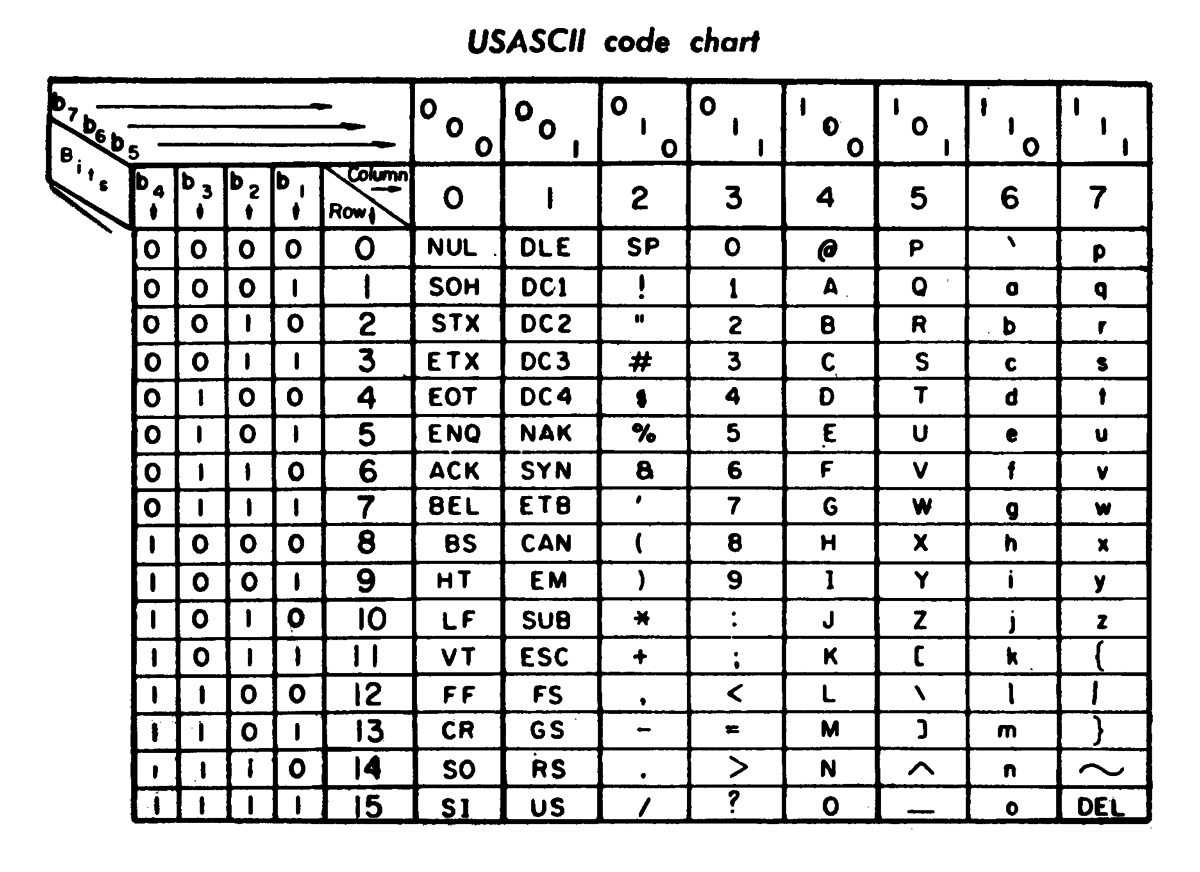
\includegraphics[width=0.5\paperwidth]{figure_man/ascii_code_chart}
\end{tabular}

{\scriptsize Source: \url{https://en.wikipedia.org/wiki/ASCII}}
\end{center}

{\footnotesize ASCII reserves the first 32 characters for control characters: codes originally intended not to represent printable information, but rather to control devices (printer etc.).
For example, the character \enquote{LF} represents a line break (\enquote{line feed}).}

\framebreak
\vspace*{-0.5cm}
\footnotesize
\begin{verbbox}
intToBits(65L)
## [1] 01 00 00 00 00 00 01 00 00 00 00 00 00 00 00 00 00 00
## [19] 00 00 00 00 00 00 00 00 00 00 00 00 00 00
\end{verbbox}
\col
\vspace{0.2cm}
\begin{verbbox}
utf8ToInt("A")
## [1] 65
\end{verbbox}
\col
\vspace{0.2cm}
\begin{verbbox}
intToUtf8(65)
## [1] "A"

coderange = c(32:126)
ascii.tab = data.frame(
  char = intToUtf8(coderange, multiple = TRUE),
  dec = coderange,
  hex = as.raw(coderange)
)
\end{verbbox}
\col
\lz
\begin{footnotesize}
Note: bit order from left to right (in contrast to the \enquote{usual} representation of binary numbers).
\end{footnotesize}

\framebreak

\footnotesize
\begin{verbatim}
head(ascii.tab, 16)
## char dec hex
## 1 32 20
## 2 ! 33 21
## 3 " 34 22
## 4 # 35 23
## 5 $ 36 24
## 6 % 37 25
## 7 & 38 26
## 8 ' 39 27
## 9 ( 40 28
## 10 ) 41 29
## 11 * 42 2a
## 12 + 43 2b
## 13 , 44 2c
## 14 - 45 2d
## 15 . 46 2e
## 16 / 47 2f
\end{verbatim}

\end{vbframe}

%\begin{vbframe}{Codes for character sets: Bit encoding}
%<<>>=
%rawToBits(charToRaw("A"))
%intToBits(65L)
%@

%\end{vbframe}

\normalsize

\begin{vbframe}{Codes for character sets: 8-bit}

There are numerous extensions from ASCII to $8$ bit for international character sets:
\begin{description}
 \item[ISO 8859 / Latin:] family of standards for different
  language groups: (1) Western Europe, (2) Eastern Europe, (3) Southern Europe, (4)
  Northern Europe, (5) Cyrillic, (6) Arabic, (7) Greek, \ldots
 \item[Windows Code Page 1252:] similar to ISO 8859; however, positions
  128-159 are not dedicated to control characters, but also used for printable characters.
\end{description}

Common problems: Sequence of bytes alone are not unique. One
needs to know which code is used. Many Asian scripts
cannot even be represented in 8 bits.
\end{vbframe}


\begin{vbframe}{Codes for character sets: unicode}
\begin{itemize}
\item Goal: a unified code-scheme for any
  languages, mathematics, music, \ldots
\item Up to $2^{32}$ characters, probably \enquote{only}
  $2^{21}$ will ever be used. Human languages use the
  first $2^{16}$ (2 bytes).
\item Defined and managed by the unicode consortium, a non-profit organization that
  all the major hardware \& software companies (Adobe, Apple, Google,
  Microsoft, Oracle, IBM, etc. ) belong to.\\


%These graphics couldnt be found in the folder of the 2014 slides
%\includegraphics[width=0.08\textwidth]{pics/adobe}
%\includegraphics[width=0.08\textwidth]{pics/apple}
%\includegraphics[width=0.08\textwidth]{pics/goap}
%\includegraphics[width=0.08\textwidth]{pics/google}
%\includegraphics[width=0.08\textwidth]{pics/ibm}
%\includegraphics[width=0.08\textwidth]{pics/microsoft}
%\includegraphics[width=0.08\textwidth]{pics/oman}
%\includegraphics[width=0.08\textwidth]{pics/oracle}
%\includegraphics[width=0.08\textwidth]{pics/sap}
%\includegraphics[width=0.08\textwidth]{pics/yahoo}
\item Close cooperation with ISO; development of standards for
  character codes are delegated to unicode.
\end{itemize}

\framebreak

  \begin{center}
    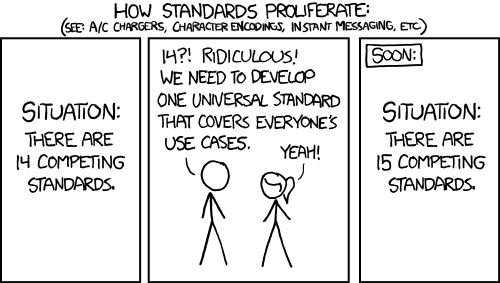
\includegraphics[width=0.8\textwidth]{figure_man/standards.png}
  \end{center}

\framebreak

Unfortunately, there are several \enquote{Unicode Transformation Formats (UTF)}.
The two most important ones are:
\begin{description}
\item[UTF-8:] the most common scheme on Unix systems. The Internet Mail Consortium (IMC) recommended that all e-mail programs should be able to display and create mail using UTF-8, and the W3C recommends UTF-8 as the default encoding in XML and HTML. 
\item[UTF-16:] older, is internally used by many \enquote{early adopters} like
  Windows NT (2000, XP, Vista, 7), Java, or Mac OS X. Not
  compatible with ASCII, since it uses 16 Bit.
\end{description}

\framebreak

UTF-8 has a variable width encoding to use 1-4 bytes:
  \begin{table}
    \begin{tabular}{llllll}
      \toprule
    Bytes & Avail. Bits & Byte 1   & Byte 2   & Byte 3   & Byte 4   \\ \midrule
    1     & 7           & 0xxxxxxx &          &          &          \\
    2     & 11          & 110xxxxx & 10xxxxxx &          &          \\
    3     & 16          & 1110xxxx & 10xxxxxx & 10xxxxxx &          \\
    4     & 21          & 11110xxx & 10xxxxxx & 10xxxxxx & 10xxxxxx \\
    \bottomrule
    \end{tabular}
  \end{table}
\begin{itemize}
  \item First bits in first byte determine the number of total bytes
  \item UTF-8 with 1 byte is compatible to ASCII
\end{itemize}

\end{vbframe}


\endlecture
\end{document}

% https://github.com/SurajGupta/r-source/blob/56becd21c75d104bfec829f9c23baa2e144869a2/src/library/stats/src/cov.c

